% \documentclass[conference]{IEEEtran}
% \documentclass[conference, onecolumn]{IEEEtran}
% <--- remove onecolumn for actual paper setup

\documentclass[letterpaper, 10 pt, conference]{ieeeconf}
\IEEEoverridecommandlockouts 
\overrideIEEEmargins

% -----------------------------------------------------
% Preamble
% -----------------------------------------------------
% Math Packages
\usepackage{physics}
\usepackage{amsmath, amssymb, empheq}
\usepackage{thmtools}
% \usepackage[per-mode=symbol]{siunitx}

% Format Packages/Settings
\usepackage{todonotes}
\usepackage{xcolor}
\usepackage[draft]{hyperref}
\renewcommand{\figureautorefname}{Fig.}

\usepackage{cite}


% Theorems
\newtheorem{definition}{Definition}
\newtheorem{theorem}{Theorem}
\newtheorem{lemma}{Lemma}
\newtheorem{corollary}{Corollary}
\newtheorem{remark}{Remark}


% Custom Commands
\newcommand{\R}{\mathbb{R}}
\newcommand{\N}{\mathbb{N}}
\newcommand{\Z}{\mathbb{Z}}
\newcommand{\st}{ \ : \ }



% Title and Author Info
\title{
    \LARGE \bf
    Optimal Combat Scenario for Dungeons \& Dragons
}

\author{
    Alyssa Vellucci and Jonas Wagner
    \thanks{
        The authors are with the Mechanical Engineering Department at the University of Texas at Dallas, Richardson, TX, USA 
    {\tt\small vellucci@utdallas.edu and jonas.wagner@utdallas.edu}
    }
}


% -----------------------------------------------------
% Begin Document
% -----------------------------------------------------
\begin{document}

% -----------------------------------------------------
% Title and Abstract
% -----------------------------------------------------
\maketitle
\begin{abstract}

    This article examines the multi-step decision-making process involved in combat encounters in Dungeons and Dragons 5th edition. 
    In D\&D combat, players fight creatures controlled by the Dungeon Master. 
    The goal is to maximize the hit points of player characters while minimizing those of the enemies. 
    The system includes the set of PCs and enemies, and the states of the system include the HP values of PCs and enemies, the condition of the PC and enemy, and spell slots remaining.

    Inputs include the actions the enemy performs and the state of the creature, while outputs include the actions the PCs perform on the enemy creature. 
    he uncertainties in this system come from the dice rolls the players make when performing an action and not knowing the specific stats of the enemy they face. 
    Combat is based on initiative order, and each round is a full completion of the initiative list.

    This system uses a Markov Decision Process to create the dynamic program.  
    This dynamic programming algorithm has been shown to be up to 70\% effective in winning these combat scenarios.


\end{abstract}


% -----------------------------------------------------
% Introduction
% -----------------------------------------------------
\section{Introduction}
The goal of this project is to create a dynamic program that can optimize a combat scenario for the game Dungeons \& Dragons. 
While the scenario the dynamic program will 
optimize is not a 1:1 representation of the D\&D 5e Ruleset, it is similar enough that it should be recognizable as a D\&D game \cite{dnd_wizards, dnd_beyond, dnd_wiki}.
Due to the sheer number of decisions that could be made in a typical D\&D combat, many limitations had to be implemented so that the program could fit within the scope of the project. 
These limiting assumptions will be outlined
in detail in \autoref{sec:pblm_def}. 

In a typical D\&D combat, characters controlled by the players (PCs) face off against enemy creatures ("monsters") controlled by the Dungeon Master (DM). The actions of PCs and creatures (collectively,
referred to as actors) are determined by a dice roll. The roll of the die plus some modifier needs to meet or exceed the so-called Armor Class (AC) to be able to count as a "hit"
and deal damage. The PCs AC is known, while the AC of the monster is hidden from the players. Only when the players roll some number and hit do they ascertain the AC of the monster.

Players can perform many actions in their turn, including melee or ranged weapon attacks, spell casts, movement on the battlefield, interaction with their environment, helping other
PCs, ingest a potion (or poison), and more. For the simulation outlined in this report, the only actions a PC can take are: move, weapon attack, drink a potion, or do nothing. Monsters 
will have the same set of actions, sans drinking a potion. The battlefield is flat with no obstacles or borders to limit movement. Both PC and monster have an AC of 15. Their strength and dexterity modifiers (used
for the sword and the bow) are +5, but this modifier is only used to determine the success of the attack, not as a modifier on the damage done to the

A combat is considered successful if the PCs live while killing the monster. Therefore, the dynamic program will be optimized to maximize the HP value of the PC, while minimizing the HP
value of the monster. 

% -----------------------------------------------------
% Problem Definition
% -----------------------------------------------------
\section{Problem Definition}\label{sec:pblm_def}
% System Definition
\subsection{Limiting Assumptions}

\begin{table}[h]
\centering
\caption{Assumptions}
\label{tab:assumptions}
\begin{tabular}{|l|p{6cm}|}
\hline
\textbf{Movement} & Single deterministic movement of 1 square per turn, followed by an action \\
\hline
\textbf{Actions} & Single action per time step: \\
& - Melee (hit check)(d6) - Short range \\
& - Ranged (hit check)(d8) - Longer range \\
& - Health Potion (d4 + 1) \\
& - Nothing \\
\hline
\textbf{Characters} & 1 PC and 1 Monster with identical specs and modifiers, using the same weapon (+2) \\
\hline
\textbf{Monster} & Moves in a standard pattern and cannot heal \\
\hline
\textbf{Time Horizon} & Infinite Time Horizon \\
\hline
\textbf{Battlefield} & Infinite with no obstacles \\
\hline
\end{tabular}
\end{table}

The assumptions for this problem are outlined above. It is important to point out that this is not a true infinite time horizon problem: the scenario does not end when converging to
some value. The simulation ends when one of the actors reaches a HP value of zero. Because it is unknown how many time steps this will take, the program is modeled like an infinite time horizon.

\subsection{Environment Definition}
\subsubsection{States}
Let each character be associated with position and HP states.
For position, let \[
    x_{pc,p}, x_{mn,p} \in \mathcal{X}_{p} \subseteq \Z^{2}
\] describe the position on an infinite 2-d grid.
For HP, let \[
    x_{pc,hp}, x_{mn,hp} \in \mathcal{X}_{hp} \subseteq \Z_+ = \{0, 1, 2, \dots\}
\] describe the HP for each character.

\subsubsection{Inputs}
The inputs to the system consist of movement and actions impacting the position and hp states respectively.
For movement, a deterministic input of 
\begin{multline}
    u_{pc,m}, u_{mn,m} \in \mathcal{U}_{m} = \text{\{0, N, E, S, W, NE, NW, SE, SW\}}\\
    =\{(0,0),(-1,0), (+1,0),(0,-1), (0,+1), \\ (-1,-1), (-1,+1), (+1,-1),(+1,+1)\}
\end{multline}

Where \(0\) is the actor not performing a movement at all.

For actions, the input for the PC and monster are respectively \[
    u_{pc,a} \in \mathcal{U}_{a} = \{\text{Melee, Ranged, Heal, Nothing}\}\]
    \[u_{mn,a} \in \mathcal{U}_{a} = \{\text{Melee, Ranged, Nothing}\}
\] where each of the actions (except nothing) are stochastic.

For Melee and Ranged attacks, the character acts upon another character's HP where the impact on HP is as follows:
\begin{enumerate}
    \item Ensure in range for either melee or ranged attack - otherwise can't attack.
    \item ``Roll'' for success/fail - if fail then self-loop on opponent HP
    \item ``Roll'' for effectiveness - opponent HP decreased by Weapon/self Modifiers (2) + d6/d8
\end{enumerate}

The PC is also allowed to use a health potion which has a stochastic effect upon the player's health:
\begin{enumerate}
    \item Ensure potion is available - otherwise can't heal
    \item ``Roll'' for effectiveness - player's HP increased by health modifier (1) + d4
\end{enumerate}

\subsubsection{Stochastic Elements}
The stochastic aspects of the system can be described as a noise signal consisting of the PC and monster dice rolls.
The actions themselves can be modeled as either a function of the noise signal or as a Markov chain acting directly upon the PC or Monster HP states.

The noise introduced by dice rolls are defined as for \{d2, d4, d6, d8, d10, d20, d100\} as 
\[
    w_{pc,dn}, w_{mn,dn} \in \mathcal{W}_{dn} = \{1,2,\dots,n\}
\] with $n = 2,4,6,8,10,20,100$ respectively where each outcome is equally likely.
The PDF can be seen in shorthand with $P(w_{i,dn} = \smqty[1 & \cdots & n]^T) = \frac{1}{n}\smqty[1 & \cdots & 1]^T$.
% 
\subsection{Simplistic System}
\subsubsection{States, Inputs, and Noise}
For the simplistic case, let states at time-step $k$, be \[
    x_k = \mqty[x_{pc,p}\\x_{mn,p}\\x_{pc,hp}\\x_{mn,hp}\\ x_{pc,potion}] 
    \in \mathcal{X} = \mathcal{X}_p^2 \cross \mathcal{X}_{hp}^2 \cross \mathcal{X}_{potion}
    \subseteq \Z^{4} \cross \Z_{+}^{2} \cross \Z_{+}
\] where states and sets are defined as before and $x_{pc,potion} \in \mathcal{X}_{potion}$ is the number of potions available to the PC.

Let the inputs to the system be only the players inputs: \[
    u_k = \mqty[u_{pc,m}\\u_{pc,a}] \in \mathcal{U} = \mathcal{U}_{p} \cross \mathcal{U}_{a} %\subseteq \{(-1,0), (+1,0), (0,-1),(0,+1), {\color{red} (-1,-1), (-1,+1), (+1,-1),(+1,+1)}\} \cross \{\text{Melee, Ranged, Heal, Nothing}\}
\] The monster's inputs to the system will be incorporated as a deterministic and stochastic input that are closed-loop within the system and treated as part of the nonlinear aspects of the update function.

Let the noise signal $w_k$ for each time-step be defined as a collection of the PC and Monster dice rolls, \[
    w_k = \mqty[w_{pc} \\ w_{mn}], \quad w_{i} = \mqty[w_{i,4} \\ w_{i,6} \\ w_{i,8} \\ w_{i,20}] \forall_{i = pc,mn}
    % \mqty[w_{pc,sf}\\w_{pc,d4}\\w_{pc,d6}\\w_{pc,d}\\w_{mn,sf}\\w_{mn,d4}\\w_{mn,d6}\\w_{mn,d8}]
\]The associated success or fail noise $\forall_{i=pc,mn} \forall_{j=mn,pc} \forall_{l = dex,str}$ is derived as \[
    w_{i,sf} = \begin{cases}
        0 & (a_{i,l} + w_{i,d20} \leq a_{j,ac})\\
        1 & (a_{i,l} + w_{i,d20} > a_{j,ac})\\
    \end{cases}
\] where the modifiers are held constant as $a_{i,l} = a_{i,dex} = a_{i,str} = 5$ and $a_{j,ac} = 15$.

\pagebreak
\subsection{System Update Equation}
The evolution of the very simple system can be described as Markov chains or by a nonlinear update function.

The nonlinear update function is as follows: \begin{multline}
    x_{k+1} = f(x_k, u_k, w_k)\\
    = \mqty[
        x_{pc,p} + f_{pc,m}(u_k)\\
        x_{mn,p} + f_{mn,m}(x_k)\\
        \mqty[x_{pc,hp}\\ x_{mn,hp} \\ x_{pc,potion}] + f_{pc,a}(x_k,u_k,w_k) + f_{mn,a}(x_k,w_k)
    ]
\end{multline}
where the associated functions update states as follows: 
\begin{itemize}
    \item The players deterministic movement input: \[
        f_{pc,m}(u_k) = u_{pc,m}
    \]
    \item The PC actions dependent on action selection and dice rolls as follows:
\end{itemize} % to return to no indent (wouldn't work for enumerate)

If $u_{pc,a} = \text{Melee} \text{ AND } \norm{x_{pc,p} - x_{mn,p}}_2 \leq a_{pc,rng,m}$, then \[
        f_{pc,a} = \mqty[0 & -w_{pc,sf}(a_{pc,wpn,m} + w_{pc,d6}) & 0]^T 
    \] 
Else if $u_{pc,a} = \text{Ranged} \text{ AND } a_{pc,rng,m} < \norm{x_{pc,p} - x_{mn,p}}_2 \leq a_{pc,rng,r}$, then \[
        f_{pc,a} = \mqty[0 & -w_{pc,sf}(a_{pc,wpn,r} + w_{pc,d8}) & 0]^T
    \]
Else if $u_{pc,a} = \text{Heal} \text{ AND } x_{pc,potion} \geq 1$, then \[
        f_{pc,a} = \mqty[a_{pc,potion} + w_{pc,d4} & 0 & -1]^T
    \]
Otherwise, $f_{pc,a} = \smqty[0 & 0 & 0]^T$

\begin{itemize} % resume the previous itemize (wouldn't work for enumerate)
    \item The monsters state-dependent movement:\[
        f_{mn,m}(x_k) = \operatorname{direction}(x_{pc,p} - x_{mn,p})
    \] where $\operatorname{direction}()$ is calculated as the closest cardinal direction that heads towards the player.
    \item The monsters state-dependent action: 
\end{itemize}

If $\norm{x_{pc,p} - x_{mn,p}}_2 \leq a_{mn,rng,m}$, then \[
    f_{mn,a} = \mqty[-w_{mn,sf}(a_{mn,wpn,m} + w_{mn,d6}) & 0 & 0]^T
\]
Else if $\norm{x_{pc,p} - x_{mn,p}}_2 \leq  a_{mn,rng,r}$, then \[
    f_{mn,a} = \mqty[- w_{mn,sf}(a_{mn,wpn,r} + w_{mn,d8}) & 0 & 0]^T
\]
Otherwise $f_{mn,a} = \smqty[0 & 0 & 0]^T$.

Weapon and potion modifiers are designed as $a_{pc,wpn,m} = a_{mn,wpn,m} = 0$, $a_{pc,wpn,r} = a_{mn,wpn,r} = 0$, and $a_{pc,potion} = 1$.
Ranges are set as $a_{pc,rng,m}= a_{mn,rng,m} = 2$ and $ a_{pc,rng,r} =  a_{mn,rng,r} = 5$.

\subsection{Markov Chain Realization}
Equivalent markov chains can be defined for each of the steps of a turn instead of the nonlinear mixed deterministic/stochastic functions. 

The relative and deterministic nature of makes those updates much easier to be done using the update function; however, the stochastic nature of actions lend well towards a markov implementation.

Transition matrices can be derived directly from the nonlinear functions for 




% -----------------------------------------------------
% Dynamic Programming Implementation
% -----------------------------------------------------
\section{Dynamic Programming Implementation}








\subsubsection{Additional assumptions}
A few additional assumptions must be made to restrict the problem to a markov chain implementation:
\begin{itemize}
    \item The monster and pc hp will be restricted to a finite range, $x_{pc,hp},x_{mn,hp} \in \mathcal{X}_{hp} = \{0,1,\dots, n_{hp,max}\}$
    \item The ensuring of a potion will be a restriction upon the pc input/result in a nothing action if no potion is available.
\end{itemize}







The objective function is defined to minimize the monsters HP and maximize the PC HP while incentivising monster death and strongly disincentivising PC death.



% Preliminaries
\subsection{Preliminaries}








% -----------------------------------------------------
% Results
% -----------------------------------------------------
\section{Results}
This process was repeated 1000 times in a Monte Carlo simulation in order to fully realize the results of the 
dynamic program. A visualizer was created to show the change of the PC and monster's states over the course of the 
combat. Fig. 1 below shows an example of the visualizer animation sequence.

\pagebreak

\begin{figure}[h]
\centering
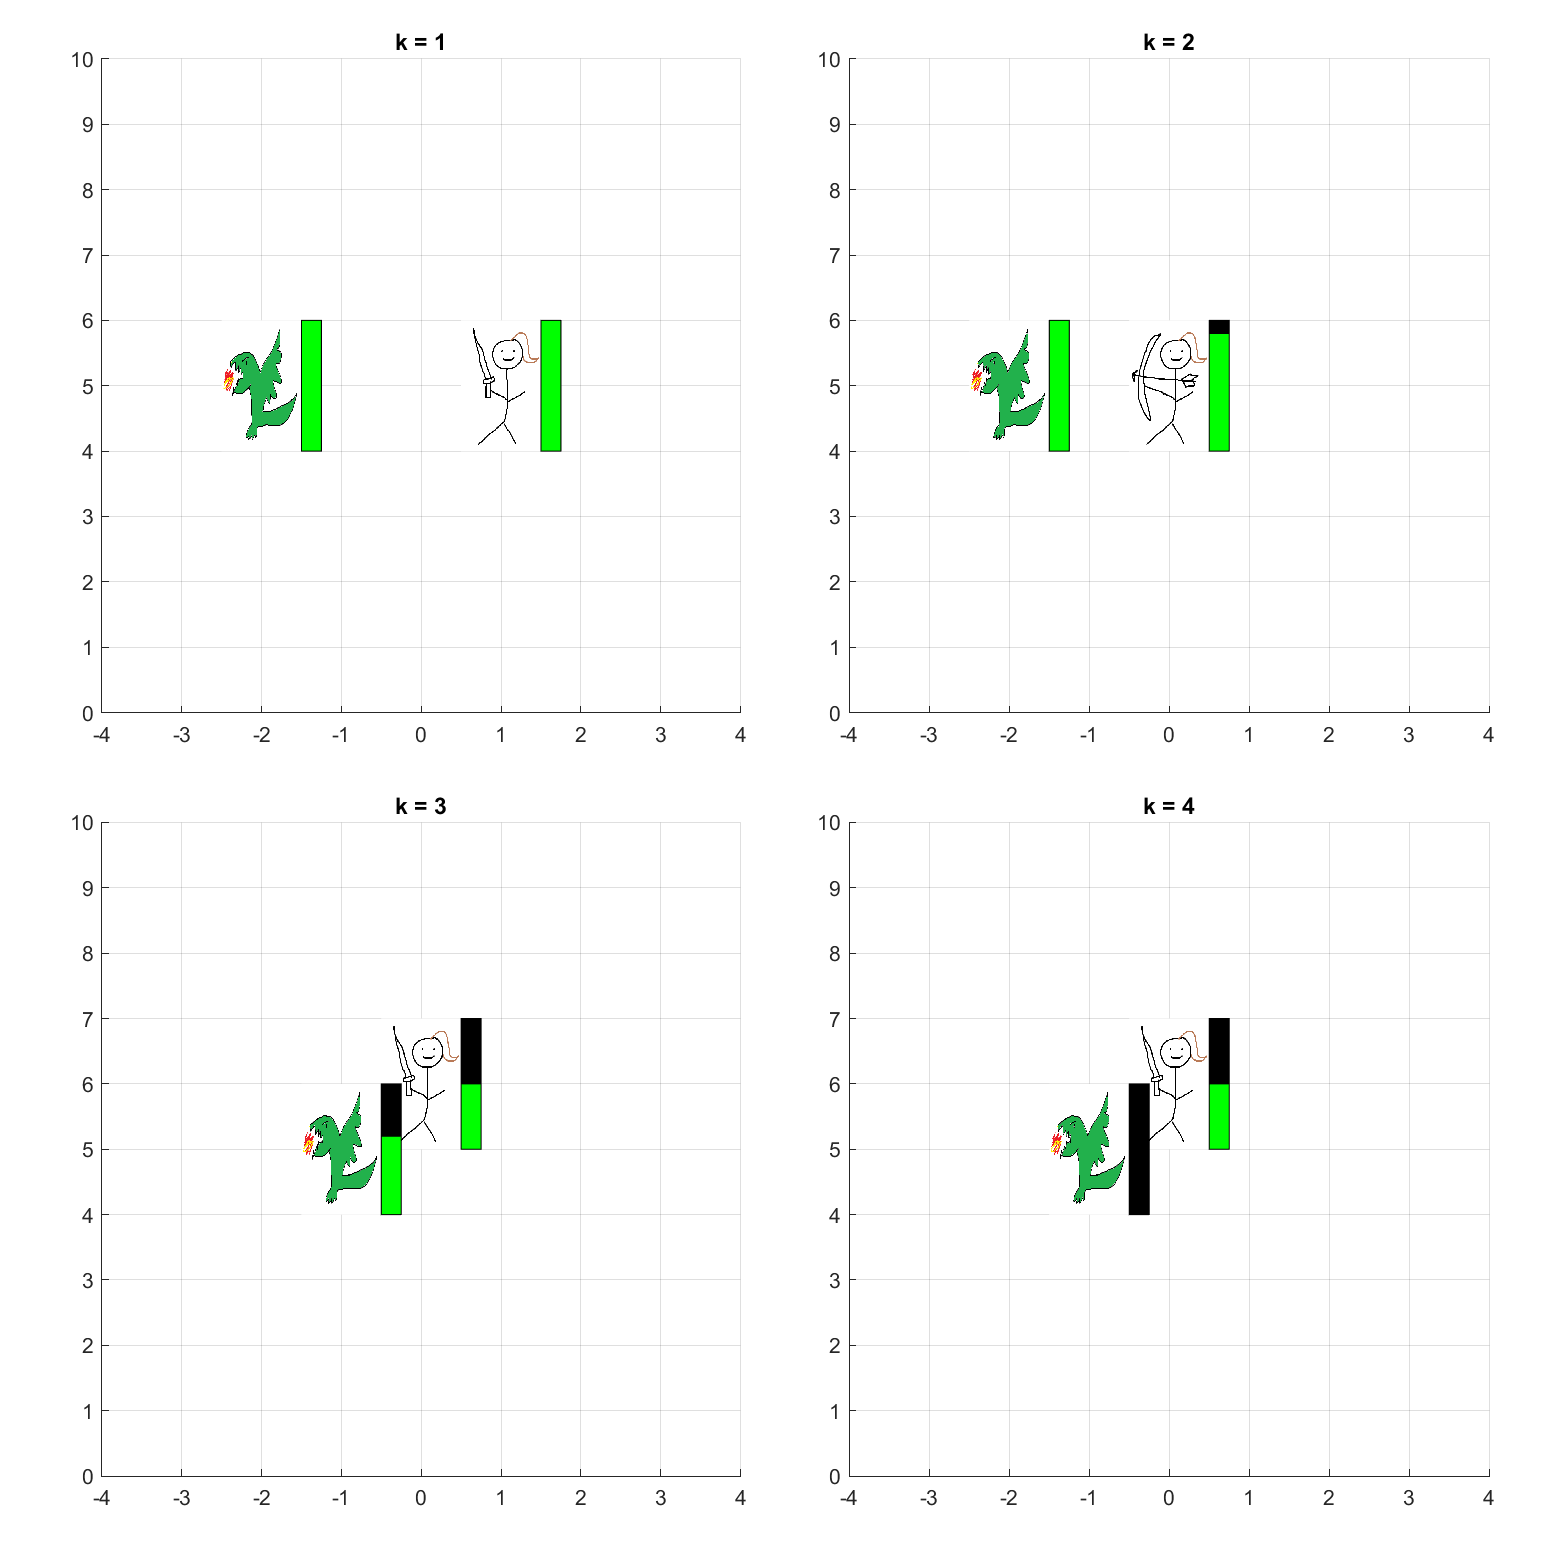
\includegraphics[scale = 0.2]{figs/DND_SingleSim_Animation_rng_seed=1997.png}
\caption{A combat scenario in which the PC defeats the monster in 4 time steps}
\end{figure}

The Monte Carlo simulation results differed depending on what computer processor was used to calculate the Markov decision 
process. Using an Intel i7-8750H (8th gen) processor, the win-rate of the PC was about 40\%, as shown in Fig. 2. Using an AMD 
Ryzen 9 3950X, the win-rate of the PC was closer to 70\%, as shown in Fig. 3. This might be due to how the processors differ in their methods of calculating
random variables, as these simulations were performed using the exact same code and random number seed.

\begin{figure}[thb]
    \centering
    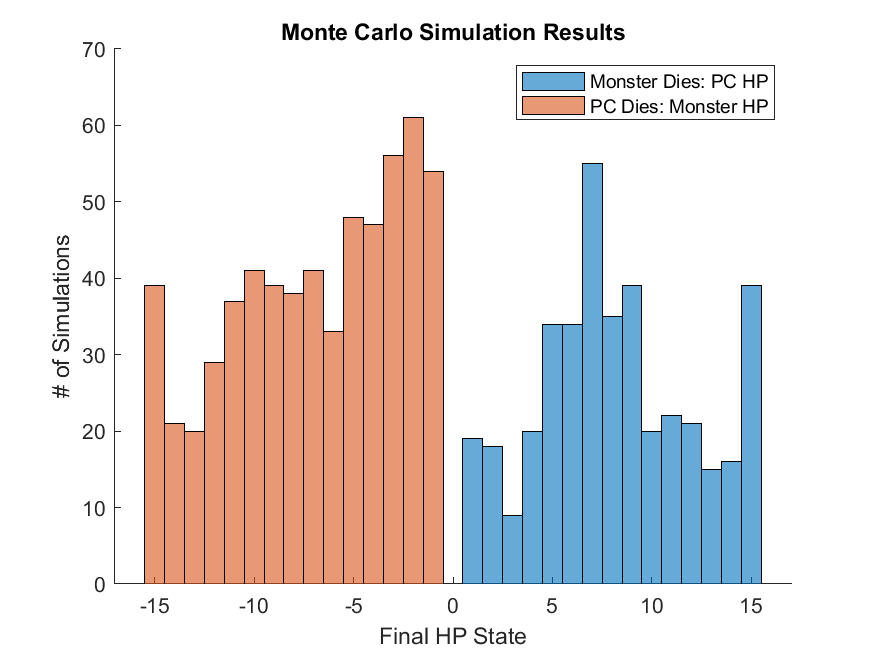
\includegraphics[scale = 0.5]{figs/DND_monte_carlo_hist.png}
    \caption{Monte Carlo simulation performed on an Intel processor.}
\end{figure}

Figures 2 and 3 depict scenarios where one of the actors dies. In some instances, both the PC and monster survive and the simulation concludes 
without a decisive outcome. This outcome could be attributed to the random positioning of the actors on the battlefield, wherein they may be too 
distant from each other, causing them to spend time running towards or away from each other instead of attacking. Alternatively, it could result 
from a sequence of unfavorable dice rolls, resulting in both parties failing to land successful hits.



\begin{figure}[thb]
    \centering
    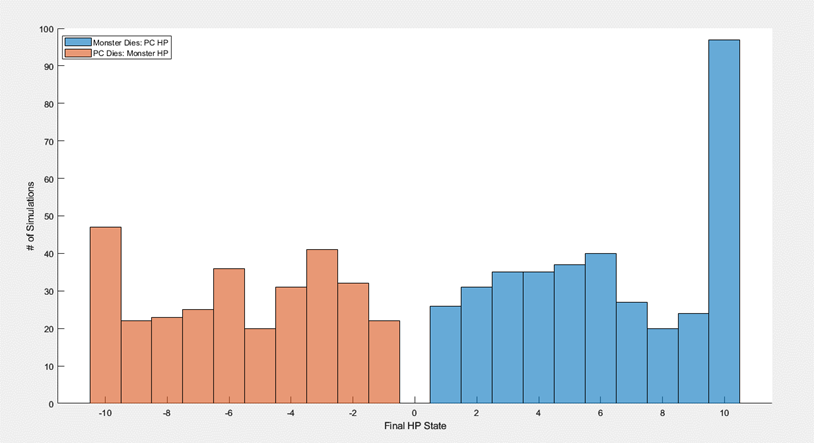
\includegraphics[width=\columnwidth]{figs/DND_MChist_AMD.png}
    \caption{Monte Carlo simulation performed on an AMD processor.}
\end{figure}

The Monte Carlo simulation results were compared to human decisions in the context of D\&D gameplay, acknowledging that the optimal choice is 
not always made by human players. In the human simulation, the PCs' actions were manually inputted while playing against the monster, and the 
findings are presented in Fig. 4. The results indicate that the human performance was superior to that of the Intel processor, 
achieving a 60\% win-rate. However, it fell short of the performance of the AMD processor.

\begin{figure}[thb]
    \centering
    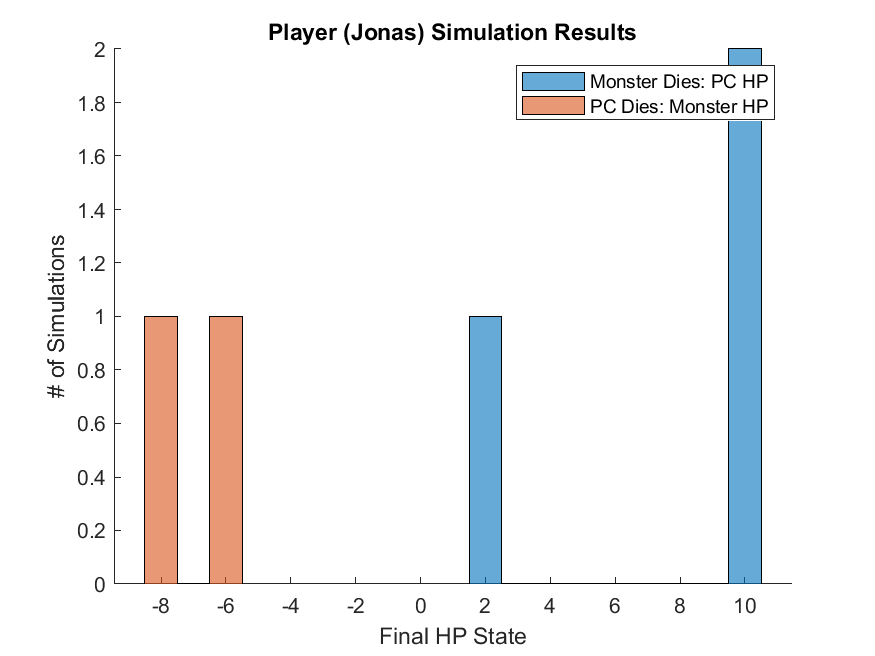
\includegraphics[scale = 0.5]{figs/DND_player_jonas_hist.png}
    \caption{Human combat results over 5 simulations.}
\end{figure}


Fig. 5 displays the stage costs of the dynamic program, with the left and bottom red bars signifying the termination of the simulation 
when the PC or monster reaches 0 HP, respectively. The objective is to maximize the PC's health while minimizing the monster's, resulting in a 
significant cost when the monster's HP is at its maximum. The program is structured to minimize negative values, effectively maximizing the highest
cost when the PC is at full health.



\begin{figure}[thb]
    \centering
    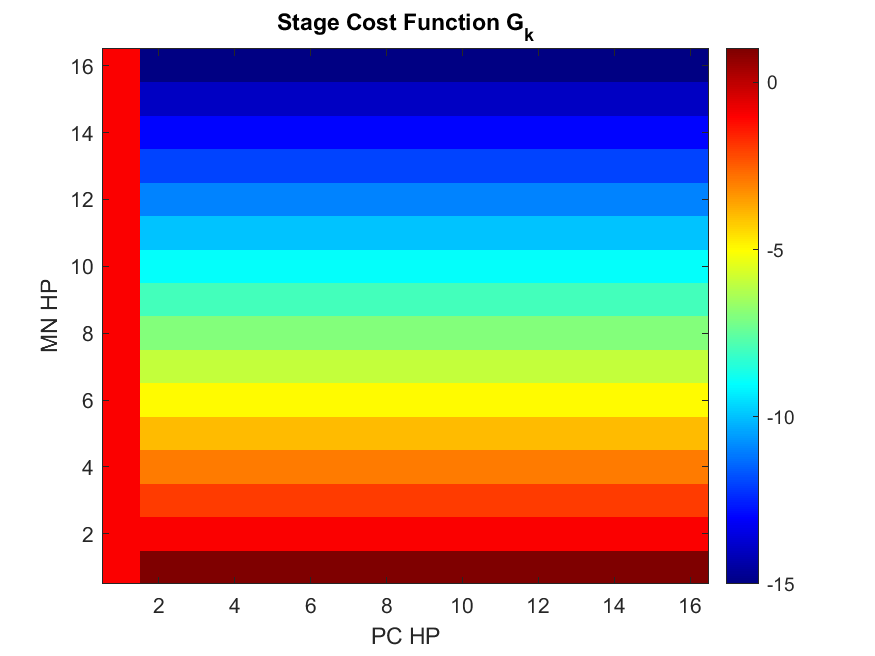
\includegraphics[scale =0.44]{figs/DND_StageCost_G_k.png}
    \caption{Stage Cost of $G_k$.}
\end{figure}



% -----------------------------------------------------
% References
% -----------------------------------------------------
\bibliography{refs}{}
\bibliographystyle{IEEEtran}




\end{document}
